\documentclass[12pt]{article}
\usepackage[margin=1in, paperwidth=8.5in, paperheight=11in]{geometry}
\usepackage{ifpdf,amsmath, amssymb, comment, color, graphicx, stmaryrd,setspace,enumerate,tikz, fancyhdr, wrapfig, textcomp, units, mathptmx, siunitx}
\usepackage{pdfpages}

\setlength{\headheight}{14.5pt}
\newcommand{\Q}{\mathbb{Q}}
\newcommand{\R}{\mathbb{R}}
\newcommand{\Z}{\mathbb{Z}}

% Solution text is in red. If you want the solutions to show, uncomment this line:
\newcommand{\red}[1]{ \textcolor{red}{#1 } }
% If you want the solutions hidden, uncomment this line:
% \newcommand{\red}[1]{ \iffalse \textcolor{red}{#1 } \fi }


\newcommand{\blue}[1]{\textcolor{blue}{#1}}
\newcommand{\green}[1]{\textcolor{green}{#1}}
\renewcommand{\section}[1]{\begin{center} \textbf{#1} \\\end{center}}
%
\setlength{\parindent}{0in}
%\oddsidemargin=-.25in
\allowdisplaybreaks
\pagestyle{fancy}
\renewcommand{\headrulewidth}{0pt}
\lhead{MATH 202}
\rhead{Spring 2025}
%\lfoot{\copyright\ CLEAR Calculus 2010}
\cfoot{}
\renewcommand{\thefootnote}{*} 
\hyphenpenalty=10000
\begin{document}
%


%\onehalfspacing
\allowdisplaybreaks
%##################################################################
\section{Physics applications of definite integrals}
\textbf{Get started:} Choose \textbf{two} of the problems below. For both problems: 
\begin{enumerate}[(a)]
\item Draw a picture of your chosen context. 
\item Explain why you can't just perform a simple multiplication to compute the requested quantity (and thus why you need a definite integral). (Hint: Something's not constant. What is it?)
\item We're interested in slicing the picture of your context into regions on which the relevant non-constant quantities are approximately constant (so that you \textit{can} just perform a simple multiplication to compute the requested quantity). Draw one representative of such a region on your picture from part A.
\end{enumerate}

\textbf{Instructions:} Work with your group on the problem you chose.
\begin{enumerate}
\item The kinetic energy of an object with mass \(m\) and constant speed \(v\) is \(K = \frac{1}{2} mv^2\), at least in the case where the entire object is moving at the same speed. Suppose a 0.1 m long rod has a mass of 0.03 kg with uniform density. It is rotating around one of its ends at a rate of one revolution per minute, much like the second hand of a clock. 
\begin{enumerate}[(a)]
\item Draw a picture. What's not constant? Draw a representative slice on which the relevant non-constant quantity is approximately constant. 

\red{The issue is that velocity is a nonconstant function of radius, $v(r)$.}
\item Compute an approximation of the kinetic energy of a representative slice, $\Delta K$.

\red{Note that the uniform density of the rod is $\frac{\SI{0.03}{kg}}{\SI{0.1}{m}} = \SI{0.3}{kg/m}$, which we'll call $\rho$.
    \[\Delta K = 1/2m(v(r))^2 = 1/2\cdot (\rho\cdot\Delta r)\cdot\left(\frac{2\pi}{60}\cdot r\right)^2, \]
where $r$ is the distance from the end of the rod to the representative slice.}
\item Write a definite integral that gives the kinetic energy of the rod in Joules (kg\(\cdot\) m\(^2\)/s\(^2\)).

\red{\[K_{total} = \int_0^{0.1} \frac{1}{2}\cdot 0.3 \left(\frac{2\pi r}{60}\right)^2\, dr\]}

\item Assign units to each factor of your integral, and describe what each factor means.
\red{
\[\int_0^{0.1} \underbrace{\frac{1}{2} \left(\underbrace{\frac{2\pi r}{60}}_{\text{Velocity of a slice at radius \(r\) (m/s)}\quad }\right)^2 \underbrace{\overbrace{0.3}^{\text{density (kg/m)}}\cdot \overbrace{dr}^{\text{thickness of slice (m)}}}_{\quad \text{mass of a slice of}\ ``\text{thickness \(dr\)" (kg)} } }_{ \text{kinetic energy of a slice of}\ ``\text{thickness \(dr\)" (J)} } \]
}

\item Assign units to each factor of your integral, and describe what each factor means.

\red{
\begin{align*} 
\int_{0}^{0.1} \frac{1}{2} \cdot 0.3 \left(\frac{2\pi r}{60} \right)^2\ dr 
& = 0.001645 \int_0^{0.1} r^2\, dr \\ 
& = 0.000548 r^3 \bigg|_0^{0.1}\\ 
& = \SI{5.483e-7}{J}
\end{align*}
So, the rod has a total energy of $\SI{5.483e-7}{J}$.}

\item If the rod is only half as long but moves twice as fast (and still has mass 30 g), does the kinetic energy increase or decrease?

\red{
Now the uniform density $\rho = \frac{\SI{0.03}{kg}}{\SI{0.05}{m}} = \SI{0.6}{kg/m}$, and the angular velocity is $\frac{2\pi}{30}$. So, our integral becomes 
\begin{align*} 
\int_{0}^{0.05} \frac{1}{2} \cdot 0.6 \left(\frac{2\pi r}{30} \right)^2\, dr 
& = 0.013159 \int_0^{0.05} r^2\ dr \\ 
& = 0.004386 r^3 \bigg|_0^{0.05}\\ 
& = \SI{5.483e-7}{J}
\end{align*}
This is actually exactly the same as the original kinetic energy!
}
\end{enumerate}
\item The density of oil in a circular oil slick on the surface of the ocean at a distance r meters from the center of the slick is given by \(\rho(r) = \frac{50}{1 + r}\) kg/m\(^2\).
\begin{enumerate}[(a)]
\item Draw a picture. What's not constant? Draw a representative slice on which the relevant non-constant quantity is approximately constant. 

\red{The issue is that density is a nonconstant function of radius, $\rho(r)$.}

\item Compute an approximation of the mass of a representative slice, $\Delta M$.

\red{
\[\Delta M = \rho(r)\cdot \Delta A = \frac{50}{1+r}\cdot (2\pi r\Delta r) \]
}
\item If the slick extends from \(r = 0\) to \(r = 10,000\) m, write a definite integral that gives the total mass of oil in the slick.

\red{
\[M_{total} = \int_0^{10000} \frac{50}{1+r}\cdot 2\pi r\, dr\]
}

\item Describe the meaning of each factor of your integral, and give its units.

\red{
\[\int_0^{10000} \underbrace{ \underbrace{\left(\frac{50}{1 + r}\right)}_{\text{Density at radius \(r\) (kg/m\(^2\))}\quad } \underbrace{2\pi r\, dr}_{\quad \text{Area of a ring at radius \(r\) with}\ ``\text{thickness \(dr\)" (m\(^2\))} } }_{ \text{Mass of oil in a ring at radius \(r\) with}\ ``\text{thickness \(dr\)" (kg)} }\]
}

\item Evaluate the integral, assign it the proper units, and explain the meaning of your result.\\
Hint: Check that \(r  - \ln(1 + r)\) is an antiderivative of $\dfrac{r}{1+r}$.

\red{
\begin{align*} 
\int_0^{10000} \frac{50}{1 + r} 2\pi r\, dr 
& = 100\pi \int_0^{10000} \frac{r}{1 + r}\ dr \\ 
&  = 100\pi (r - \ln(1 + r)) \bigg|_0^{10000}\\ 
& = 100\pi(10000 - \ln(10001))\\ & = \SI{3.1386e6}{kg}
\end{align*}
So, the total mass of the slick is $\SI{3.1386e6}{kg}.$
}

\item Is more than half, or less than half, of the oil contained within a 5,000 m radius? 
\red{
\begin{align*} 
\int_0^{5000} \frac{50}{1 + r} 2\pi r\, dr 
& = 100\pi \int_0^{5000} \frac{r}{1 + r}\ dr \\ 
&  = 100\pi (r - \ln(1 + r)) \bigg|_0^{5000}\\ 
& = 100\pi(5000 - \ln(5001))\\ & = \SI{1.56812e6}{kg}
\end{align*}This is slightly less than half of the oil.
}
\end{enumerate}

\item The force of gravity that the earth exerts on an object diminishes as the object gets further away from the earth. The energy required to lift an object 1 foot at sea level is greater than the energy required to lift the same object 1 foot at the top of Mt. Everest. However, the difference in altitudes is so small in comparison to the radius of the earth that the difference in energy is negligible. On the other hand, when an object is rocketed into space, the fact that the force of gravity diminishes with distance from the center of the earth is critical. According to Newton, the force of gravity on a given mass is proportional to the reciprocal of the square of the distance of that mass from the center of the earth. That is, for some constant \(k\), the gravitational force at distance \(r\) from the center of the earth is given by 
\[ F(r) = \frac{k}{r^2}.\]
The energy required to move an object a distance \(d\) is \(E = F\cdot d\), if the force is constant over the distance \(d\).  
\begin{enumerate}[(a)]
\item Draw a picture. What's not constant? Draw a representative slice on which the relevant non-constant quantity is approximately constant. 

\red{The issue is that force is a nonconstant function of radius, $F(r)$.}

\item Compute an approximation of the energy required to move through a representative slice, $\Delta E$.

\red{
\[\Delta E = F(r)\cdot d = \frac{k}{r^2}\cdot\Delta r\]
}
\item Write a definite integral that gives the energy in Joules (1 J = 1 N$\cdot$m) required to lift a 1-kg payload from the surface of the earth to the moon, which is about 362,570 km away at its closest point.

\red{
\[E_{total} = \int_{6371000}^{362570000}\frac{k}{r^2}\,dr\]
}

\item Assign units to each factor of your integral, and describe what each factor means.

\red{
\[\int_{6371000}^{362570000} \underbrace{ \underbrace{\frac{k}{r^2} }_{\text{Force required at \(r\) (N)}\quad } \underbrace{dr}_{\quad \text{Distance moved (m)} } }_{ \text{Energy to move the 1 kg payload a distance \(dr\) (J)}} \]
}

\item Evaluate the integral, assign it the proper units, and explain the meaning of your result.\\
(Hint: The earth's surface is at a distance of 6,371 km from its center. At this value of \(r\), the force of gravity on the 1 kg object is 9.8 N. Use this to determine the constant \(k\).)

\red{
    First, let's find the value of $k$:
    \[9.8 = F(6371000) = \frac{k}{(6371000)^2} \text{, so } k = (6371000)^2\cdot 9.8 \approx \num{3.9778e14}. \]
    Now we can find the value of the integral (but I'll leave $k$ as a letter until the very end):
\begin{align*}
E_{total} &= \int_{6371000}^{362570000}\frac{k}{r^2}\,dr = \frac{-k}{r}\bigg|_{6371000}^{362570000} 
= -k\left(\frac{1}{362570000} - \frac{1}{6371000}\right) \\
&= -k\cdot\num{-1.54203e-7} = \num{3.9778e14}\cdot\num{1.54203e-7} = \SI{6.1339e7}{J}.
\end{align*}
So, the total energy required to move the payload to the moon is  $\SI{6.1339e7}{J}$.
}

\item How far can the 1-kg payload be lifted using half the energy required to take it to the
moon? 
\red{
\[
\int_{6371000}^{D}\frac{k}{r^2}\,dr = \left.\frac{-k}{r}\right|_{6371000}^{D}
= -k\left(\frac{1}{D} - \frac{1}{6371000}\right).
\]
Setting this value equal to $\frac{1}{2} \cdot \SI{6.1339e7}{J} = \SI{6.1339e7}{J} = \SI{3.06695e7}{J}$, inserting the value of $k$, and solving for $D$ gives $D = \SI{12521870}{m}$. This is $\SI{12552}{km}$ from the center of the earth, which is $\SI{6151}{km}$ off the ground. Interestingly, this is only about 1/59\textsuperscript{th} of the distance to the moon!
}

\end{enumerate}
\item The energy required to move an object a distance \(x\) while exerting a constant force \(F\) is \(E = Fx\).  Suppose that you have two magnets and a wire. One magnet is attached to the end of the wire and the other can slide along the wire. If the magnets are arranged so that they repel each other, then it will require force to push the movable magnet toward the fixed magnet. The amount of force needed to move the magnet increases as the two get closer together. In fact, the force at a distance \(x\) is proportional to \(1/x^2\); that is, for some constant $k$, the force at a distance $x$ is $k\cdot 1/x^2$.
\begin{enumerate}[(a)]
\item Draw a picture. What's not constant? Draw a representative slice on which the relevant non-constant quantity is approximately constant. 

\red{The issue is that force is a nonconstant function of distance, $F(x)$.}

\item Compute an approximation of the energy required to move through a representative slice, $\Delta E$.

\red{
\[\Delta E = F(x)\cdot d =  \frac{k}{x^2}\cdot\Delta x\]
}
\item Write a definite integral that gives the energy required to move the magnet from 5 cm away to 3 cm away in Joules (kg\(\cdot\)m\(^2\)/s\(^2\)).

\red{
\[E_{total} = \int_{0.03}^{0.05} \frac{k}{x^2}\,dx\]
}

\item Assign units to each factor of your integral, and describe what each factor means.

\red{
\[\int_{0.03}^{0.05} \underbrace{ \underbrace{\frac{k}{x^2}}_{\text{Force required to move magnet at distance \(x\) (N)}\quad } \underbrace{dx}_{\text{Distance moved (m)} } }_{ \text{Energy required to move the magnet a distance \(dx\) when the magnets are \(x\) m apart (J)} }\]
}

\item Evaluate the integral, assign it the proper units, and explain the meaning of your result.

\red{
\[E_{total} = \int_{0.03}^{0.05} \frac{k}{x^2}\,dx = \frac{-k}{x}\bigg|_{0.03}^{0.05} = k\cdot\SI{13.33}{J}\]
So, it takes 13.33$k$ J (not to be confused with 13.33 kilojoules!) to move the magnet this distance.
}

\item Which will require more energy, to move the magnet from 5 cm away to 3 cm away, or from 3 cm away to 2 cm away?

\red{\[\int_{0.02}^{0.03} \frac{k}{x^2}\,dx = \frac{-k}{x}\bigg|_{0.02}^{0.03} = k\cdot\SI{16.67}{J},\] so it takes more energy to move from 3cm away to 2cm away.}
\end{enumerate}
\item An exponential model for the density of the earth's atmosphere says that if the temperature of the atmosphere were constant, then the density of the air as a function of height, \(h\) (in meters), above the surface of the earth would be given by
\[ \rho(h) = 1.28 e^{-0.000124 h} \text{ kg/m}^3.\]
\begin{enumerate}[(a)]
\item Draw a picture. What's not constant? Draw a representative slice on which the relevant non-constant quantity is approximately constant. 

\red{The issue is that density is a nonconstant function of height, $\rho(h)$.}

\item Compute an approximation of the mass of a representative slice, $\Delta M$.

\red{
First, since the slice is a very thin spherical "shell", we can approximate its volume as its surface area times its thickness: $\Delta V \approx 4\pi r^2\cdot \Delta r$. (Think about painting a basketball.)
\[\Delta M = \rho(h) \cdot \Delta V = 1.28 e^{-0.000124 h} \cdot 4\pi r^2 \Delta r.\]
Now, I'm irritated that this involves both $h$ and $r$, so note that $h = r - 6400000$ (since the radius of the earth is about $\SI{6400}{km}$):
\[\Delta M = 1.28 e^{-0.000124 (r - 6400000)} \cdot 4\pi r^2\Delta r.\]
}
\item Write a definite integral that gives the mass of the portion of the atmosphere from \(h = 0\) to  \(h = 100\) m (i.e., the first 100 meters above sea level). Assume the radius of the earth is 6400 km. Use a computer algebra system such as Wolfram Alpha or Geogebra to find an antiderivative.

\red{
Note that $h = 0$ corresponds to $r = 6400000$ and $h = 100$ corresponds to $r = 6400100$.
\[M_{total} = \int_{6400000}^{6400100} 1.28 e^{-0.000124 (r - 6400000)} \cdot 4\pi r^2\,dr\]
}

\item Assign units to each factor of your integral, and describe what each factor means.

\red{
\[\int_{6400000}^{6400100} 
    \underbrace{ 
        \underbrace{ 1.28 e^{-0.000124(r-6400000)} }_
            { \stackrel{ \text{Density of the earth's atmosphere}}
                       { \text{at altitude $r$ (kg/m\(^2\))   }\quad } } 
        \underbrace{ 4\pi r^2\ dr }_
            { \stackrel{ \text{Volume of a thin shell of the earth's} }
                       { \text{atmosphere at altitude $r$ (m\(^3\))} } } }
    _{ \text{Mass of a spherical shell with thickness \(dr\) of the earth's atmosphere 
            at altitude $r$ (kg)} }\]
}

\item Evaluate the integral, assign it the proper units, and explain the meaning of your result.

\red{
\begin{align*}
M_{total} &= 1.28 \cdot 4\pi \int_{6400000}^{6400100} e^{-0.000124 (r - 6400000)} r^2\,dr \\
&= 5.12\pi \int_{6400000}^{6400100} e^{-0.000124 r + 793.6} r^2\,dr \\
&= 5.12\pi\cdot e^{793.6} \int_{6400000}^{6400100} e^{-0.000124r} r^2\,dr \\
&= 5.12\pi\cdot e^{793.6} \left[\frac{-e^{-0.000124 r} \left((-0.000124)^2 r^2 + 2(-0.000124) r + 2\right)}
                                     {(-0.000124)^3}
                          \right|_{6400000}^{6400100} \\
&= \SI{6.5478e16}{kg}.
\end{align*}
So, there is about $\SI{6.5478e16}{kg}$ of air in the first 100 meters of the atmosphere.
}

\item Use this model to compute the total mass of the earth's atmosphere. According to NASA, the atmosphere is about 60 miles thick. Use WolframAlpha to calculate because these numbers are yucky.

\red{
60 miles is approximately 96560 meters. Therefore, we're changing the upper bound of our definite integral from 6400100 to $6400000 + 96560 = 6496560$.\[M_{total} = \int_{6400000}^{6496560} 1.28 e^{-0.000124 (r - 6400000)} \cdot 4\pi r^2\,dr = \SI{5.326e18}{kg}.\]}
\end{enumerate}
\item The gravitational attraction between two particles of mass \(m_1\) and \(m_2\) at a distance \(r\) apart is
\[F(r) = \frac{Gm_1 m_2}{r^2}.\]
We'll use this to find the gravitational attraction between a thin uniform rod of mass $M$ and length $l$ and a particle of mass $m$ lying in the same line as the rod at a distance $a$ from one end.
\begin{enumerate}[(a)]
\item Draw a picture. What's not constant? Draw a representative slice on which the relevant non-constant quantity is approximately constant. 

\red{The issue is that force is a nonconstant function of radius, $F(r)$.}

\item Compute an approximation of the gravitational force exerted by a representative slice, $\Delta F$.

\red{
First, let's compute the mass of the slice, $\Delta M$. Since the rod has total mass $M$ and total length $l$, the mass density is $\dfrac{M}{l}$. Therefore, a slice of length $\Delta r$ has mass $\Delta M = \dfrac{M}{l}\cdot\Delta r$.
\[\Delta F = \frac{G\cdot m \cdot \Delta M}{r^2} = \frac{G\cdot m}{r^2}\cdot\frac{M}{l}\cdot\Delta r\]
}
\item Write a definite integral that that gives the gravitational attraction between a thin uniform rod of mass \(M\) and length \(l\) and a particle of mass \(m\) lying in the same line as the rod at a distance $a$ from one end.

\red{
\[F_{total} = \int_a^{a+l} \frac{G\cdot m}{r^2}\cdot\frac{M}{l}\, dr\]
}

\item Assign units to each factor of your integral, and describe what each factor means.

\red{
\[\int_{a}^{a+I} \underbrace{ \frac{Gm}{r^2} \underbrace{\frac{M}{l}dr}_{\quad \text{mass of a slice of the rod of thickness \(dr\) (kg)} } }_{ \stackrel{\text{Gravitational force between the point of mass \(m\) and a} }{\text{slice of the rod of thickness \(dr\) separated by \(r\) meters (N)} } }\]
}

\item Evaluate the integral, assign it the proper units, and explain the meaning of your result.

\red{
\begin{align*}
F_{total} &= \int_a^{a+l} \frac{G\cdot m}{r^2}\cdot\frac{M}{l}\, dr 
= \frac{G\cdot m\cdot M}{l} \int_a^{a+l} \frac{1}{r^2}\,dr \\
&= \frac{GMm}{l}\cdot\left[\frac{-1}{r}\right|_a^{a+l} 
 = \frac{GMm}{l}\left(\frac{1}{a} - \frac{1}{a+l}\right) * \\
&= \frac{GMm}{l}\cdot\left(\frac{a+l-a}{a(a+l)}\right) 
 = \frac{GMm}{a(a+l)} \si{N}.
\end{align*}
(Keep an eye on that starred line for future reference.)
}

\item Two long, thin, uniform rods of length $l_1$ and $l_2$ lie on a straight line with a gap between them of length $A$. Suppose their masses are $M_1$ and $M_2$, respectively. What is the force of attraction between the rods? (Use the results of the previous parts.) 
\red{
If the gravitational force between a point mass of mass $m$ and a rod of length $l$ separated by a distance of $a$ is 
$\dfrac{GMm}{l}\left(\dfrac{1}{a} - \dfrac{1}{a+l}\right)$ (the starred equation from part (d)), then the force on a representative slice of rod 2 (which we can think of as a point mass) is 
\[\Delta F = \dfrac{GM_1}{l_1}\left(\dfrac{1}{r} - \dfrac{1}{r+l_1}\right)\cdot \dfrac{M_2}{l_2}\, \Delta r,\]
because now the separation distance should be a variable $r$, which should range from $A$ to $A+l_2$ (ie., from the closer end of the second rod to the further end), and the $m$ in the starred equation from part (d) should be replaced by the expression for the mass of the slice, which is $\dfrac{M_2}{l_2}\,\Delta r$.\\
Therefore, the total force is given by integrating this expression for the force on a slice: 
\begin{align*}
\int_A^{A+l_2} \frac{GM_1 M_2}{l_1 l_2}\left(\frac{1}{r} - \frac{1}{r+l_1}\right)\, dr
& = \frac{GM_1 M_2}{l_1 l_2}\left[\ln{r}-\ln{(r+l_1)}\right|_A^{A+l_2} \\
&= \frac{GM_1 M_2}{l_1 l_2}\left[\ln{\frac{r}{r+l_1}}\right|_A^{A+l_2} \\
&= \frac{GM_1 M_2}{l_1 l_2} 
\left[\ln{\frac{A+l_2}{A + l_2 + l_1}} - 
      \ln{\frac{A}{A+ l_1}}\right] \\
&= \frac{GM_1 M_2}{l_1 l_2} \left[\ln{\frac{(A+l_2)(A+l_1)}{(A)(A+l_2+l_1)}}\right] \si{N}.
\end{align*}
}
\end{enumerate}
\end{enumerate}
\red{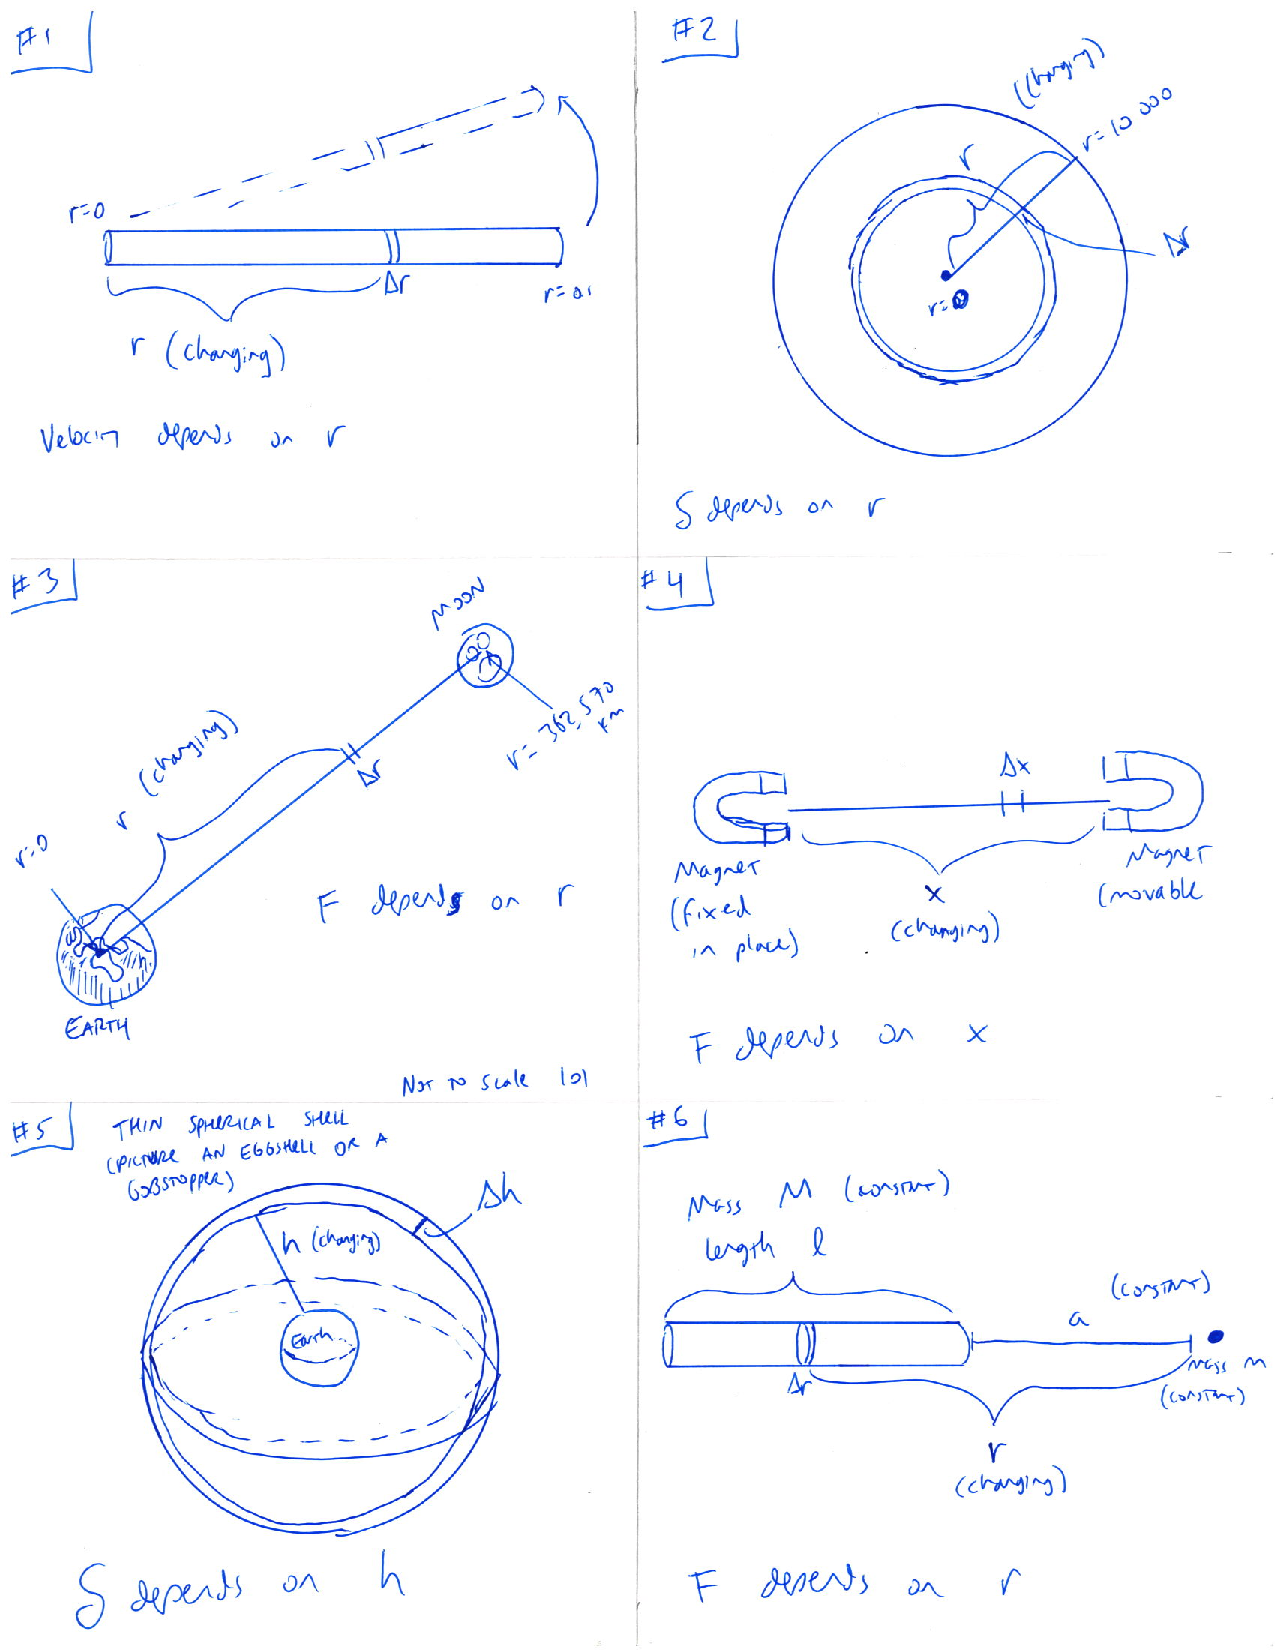
\includepdf[fitpaper=true]{images/physics-applications-diagrams.pdf}}
\end{document}